\section{Introduction}
\subsection{Motivation and Background}
Since the publication of the Fortran 2008 standard in 2010~\cite{iso2010information}, Fortran supports a \gls{spmd}
programming style that facilitates the creation of a fixed number of replicas of a compiled program, wherein each replica
executes asynchronously after creation.  Fortran refers to each replica as an image.  The primary mechanism for distributing and
communicating data between images involves defining \glspl{coarray}, entities that may be referenced or defined on one image by
statements executing on other images.  As such, a coarray defines a \gls{pgas} in which one image referencing or defining a
coarray on another image causes inter-image communication.

The seminal role that \glspl{coarray} played in the development of Fortran's intrinsic parallel programming model have made it
common to refer to all of modern Fortran's parallel programming features under the rubric of \gls{caf}.  To date, most
published \gls{caf} applications involve scenarios wherein the parallelization itself poses one of the chief
challenges and necessitates the custom development of parallel algorithms.  These include ordinary and partial differential
equation solvers in domains ranging from nuclear fusion~\cite{preissl2011multithreaded} and
weather~\cite{mozdzynski2015partitioned} to multidimensional fast Fourier transforms and multigrid numerical
methods~\cite{garain2015comparing}.  Much of the effort involved in
expressing parallel algorithms for these domains centers on
 designing and using various \gls{coarray} data structures.  In such settings, the moniker
\gls{caf} seems appropriate.

Less widely appreciated are the ways in which Fortran's intrinsic parallel programming model supports embarassingly parallel
applications, wherein the division into independent sub-problems requires little or no coordination between the
the sub-problems. To support such applications, a parallel programming
model might provide for explicit sub-problem disaggregation and independent sub-problem execution without any need for \glspl{coarray}.  The upcoming Fortran 2015 standard
(expected to be published in 2018\footnote{A Committee Draft is at https://bit.ly/fortran-2015-draft.}) will provide several
features that enable a considerable amount of parallel computation, coordination, and even some data communication
without the use of \glspl{coarray}.  In the context of \gls{caf}, we propose a working definition of ``embarassingly parallel''
as denoting the class of parallel applications for which Fortran's non-\gls{coarray} parallel features cover all of the
application's parallel algorithmic needs.

Fortran's non-\gls{coarray} parallel features include
\begin{itemize}
   \item the ability to form teams of images that communicate only with each other by default,
   \item mechanisms for ordering program segments in differing images (image synchronization),
   \item collective subroutines containing highly optimized implementations of common parallel
         communication and computation patterns;
   \item functions that return an image identifier and the number of images.
   \item global error termination.
\end{itemize}
We anticipate that a common use case for these capabilities will involve running an ensemble of simulations, each member of
which executes in a separate team.  This paper presents such a use case in the context of \gls{wrf-hydro}, a terrestrial
hydrological model developed at \gls{ncar}.


\subsection{Objectives}\label{sec:objectives}
The objectives of the current work are threefold:
\begin{enumerate}
  \item To contribute the first-ever compiler front-end support for Fortran 2015 teams.
  \item To contribute the parallel runtime library functionality required to support the new compiler capabilities.
  \item To study and address issues arising form integrating teams into an existing \gls{mpi} application, \gls{wrf-hydro},
        for purposes of driving ensembles of simulations.
\end{enumerate}
The compiler front-end described in this paper lives on the teams branch of the
\fnurl{Sourcery Institute \gls{gcc} fork}{https://github.com/sourceryinstitute/gcc}. The parallel runtime libary lives on the
opencoarrays-teams branch of the \fnurl{OpenCoarrays \gls{abi}}{https://github.com/sourceryinstitute/opencoarrays}.

The remainder of this paper is organized as follows: Section~\ref{sec:methodology} provides an overview of teams and their
support in the aforementedioned \gls{gcc} fork and in OpenCoarrays.  Section~\ref{sec:discussion} discusses the use of teams
in \gls{wrf-hydro} and a required language extension. Section~\ref{sec:conclusions} summarizes our conclusions and plans for
future work.

\section{Methodology}\label{sec:methodology}
\subsection{Teams in Fortran 2015}\label{teams-in-fortran-2015}
The Fortran 2008 parallel programming features do not provide for an environment in which
subset of the images can easily work on part of an application without affecting
other images in the program.  Grouping the images of a program into nonoverlapping
teams allows one to execute more effectively and independently parts of a larger
problem.  A class of problems that can benefit from this feature is multiphysics codes
(e.g.,  climate models).
Such a feature, called \textit{Teams} in the Committee Draft of the Fortran 2015 standard, can significantly
reduce the amount of off-node communication on an exascale machine, in particular when an entire team of images
fits within a single compute node.
The authors are unaware of any compiler support for this new feature other than that developed in the aforementioned
\gls{gcc} fork and \gls{abi} branch developed for the current project.  The remainder of the current section
provides an overview of the \textit{Teams} concept, the associated languager syntax, and the the compiler/\gls{abi}
implementation.

A team is a set of images that can readily execute independently of other images outside the team.
At program launch, all images comprise a team designated by a language-defined integer identifier \texttt{initial\_team}.
Except for the initial team, every team has a parent team assigned in a one-to-many parent/child hierarchy.
A program executes a \texttt{form team} statement to divide the current team into new child teams.
Each new team has an integer identifer that Fortran produces as the result of invoking the \texttt{team\_number()}
intrinsic function.  Information about the team to which the current image belongs can be determined by the
processor from the collective value of the team variables on the images of the team.
All images execute the \texttt{form team} statement as a collective operation.

During execution, each image has a current team, which is only changed by execution of \texttt{change team} and
\texttt{end team} statements. Executing \texttt{change team} moves the executing image form the current team to a team
specified by a variable of derived type~\texttt{team\_type}.  Subsequent execution of a corresponding \texttt{end team}
statement restores the current team back to that team to which it belonged immediately prior to execution of the most
recent \texttt{change team} statement.

Teams are described by a scalar, derived type variable of type \texttt{team\_type}. This derived-type variable has private components.
The \texttt{form team} statement takes as first argument a \texttt{team\_number} that uniquely identifies the team and a \texttt{team\_type}
variable as second argument.
Successful execution of a \texttt{form team} statement assigns the team-variable (of type \texttt{team type}) on each
participating image a value that specifies the new team that the image will belong to.
The \texttt{change team} statement takes as argument a \texttt{team type} variable that represents the new team to be used as
current team. The execution of the \texttt{end team} statement restores the current team back
to that immediately prior to execution of the \texttt{change team} statement.

\subsection{Teams in \gls{gcc} and OpenCoarrays}\label{subsec:teams-in-gcc}
From an MPI perspective, a Fortran team is comparable to an MPI communicator. The \texttt{form team} statement is implemented in OpenCoarrays
using \texttt{MPI\_Comm\_split} and passing the team id argument as \texttt{color} for \texttt{MPI\_Comm\_split}.
In case of success, the resulting communicator is stored into a list of available teams.
Every element of the list keeps track of the association of team identifier and a MPI communicator.
The elements of the list of available teams gets returned by the function and stored into the \texttt{team type} variable.

The list of available and used teams are both initialized to team 1 (equivalent to \texttt{MPI\_COMM\_WORLD}) at the beginning of the execution.
When the \texttt{change team} statement gets invoked, the element of the list of available teams stored into the \texttt{team\_type} variable
gets passed as argument to the correspondent OpenCoarrays function. The \texttt{current\_team} variable used inside OpenCoarrays for
representing the current communicator gets reassigned with the value contained into the element of the list passed as argument.
Finally, a new element is added to the list of used teams. This list of element is nothing but a list of pointers to the elements of the list
of available teams. The insertion operation is always performed at the beginning of the list in order to keep track of the teams hierarchy.
An execution of the \texttt{end team} statements is implemented by removing the first element of the list of used teams and reassigning the
\texttt{current team} to the new first element of the list of used teams.

Figure~\ref{fig:teams} depicts schematically an initial team of images (black arrows) executing over time (progressing
downward) and able to coordinate and communicate through a global mechanism (black horizontal line).  At the point of executing
\texttt{form team} and \texttt{change team} statements, the compiler inserts references to the OpenCoarrays \gls{abi} into the
executable program.  Those references cause invocations of \texttt{MPI\_Split}, which in turn creates the colored groupings that
correspond to teams in Fortran 2015.

\begin{figure*}
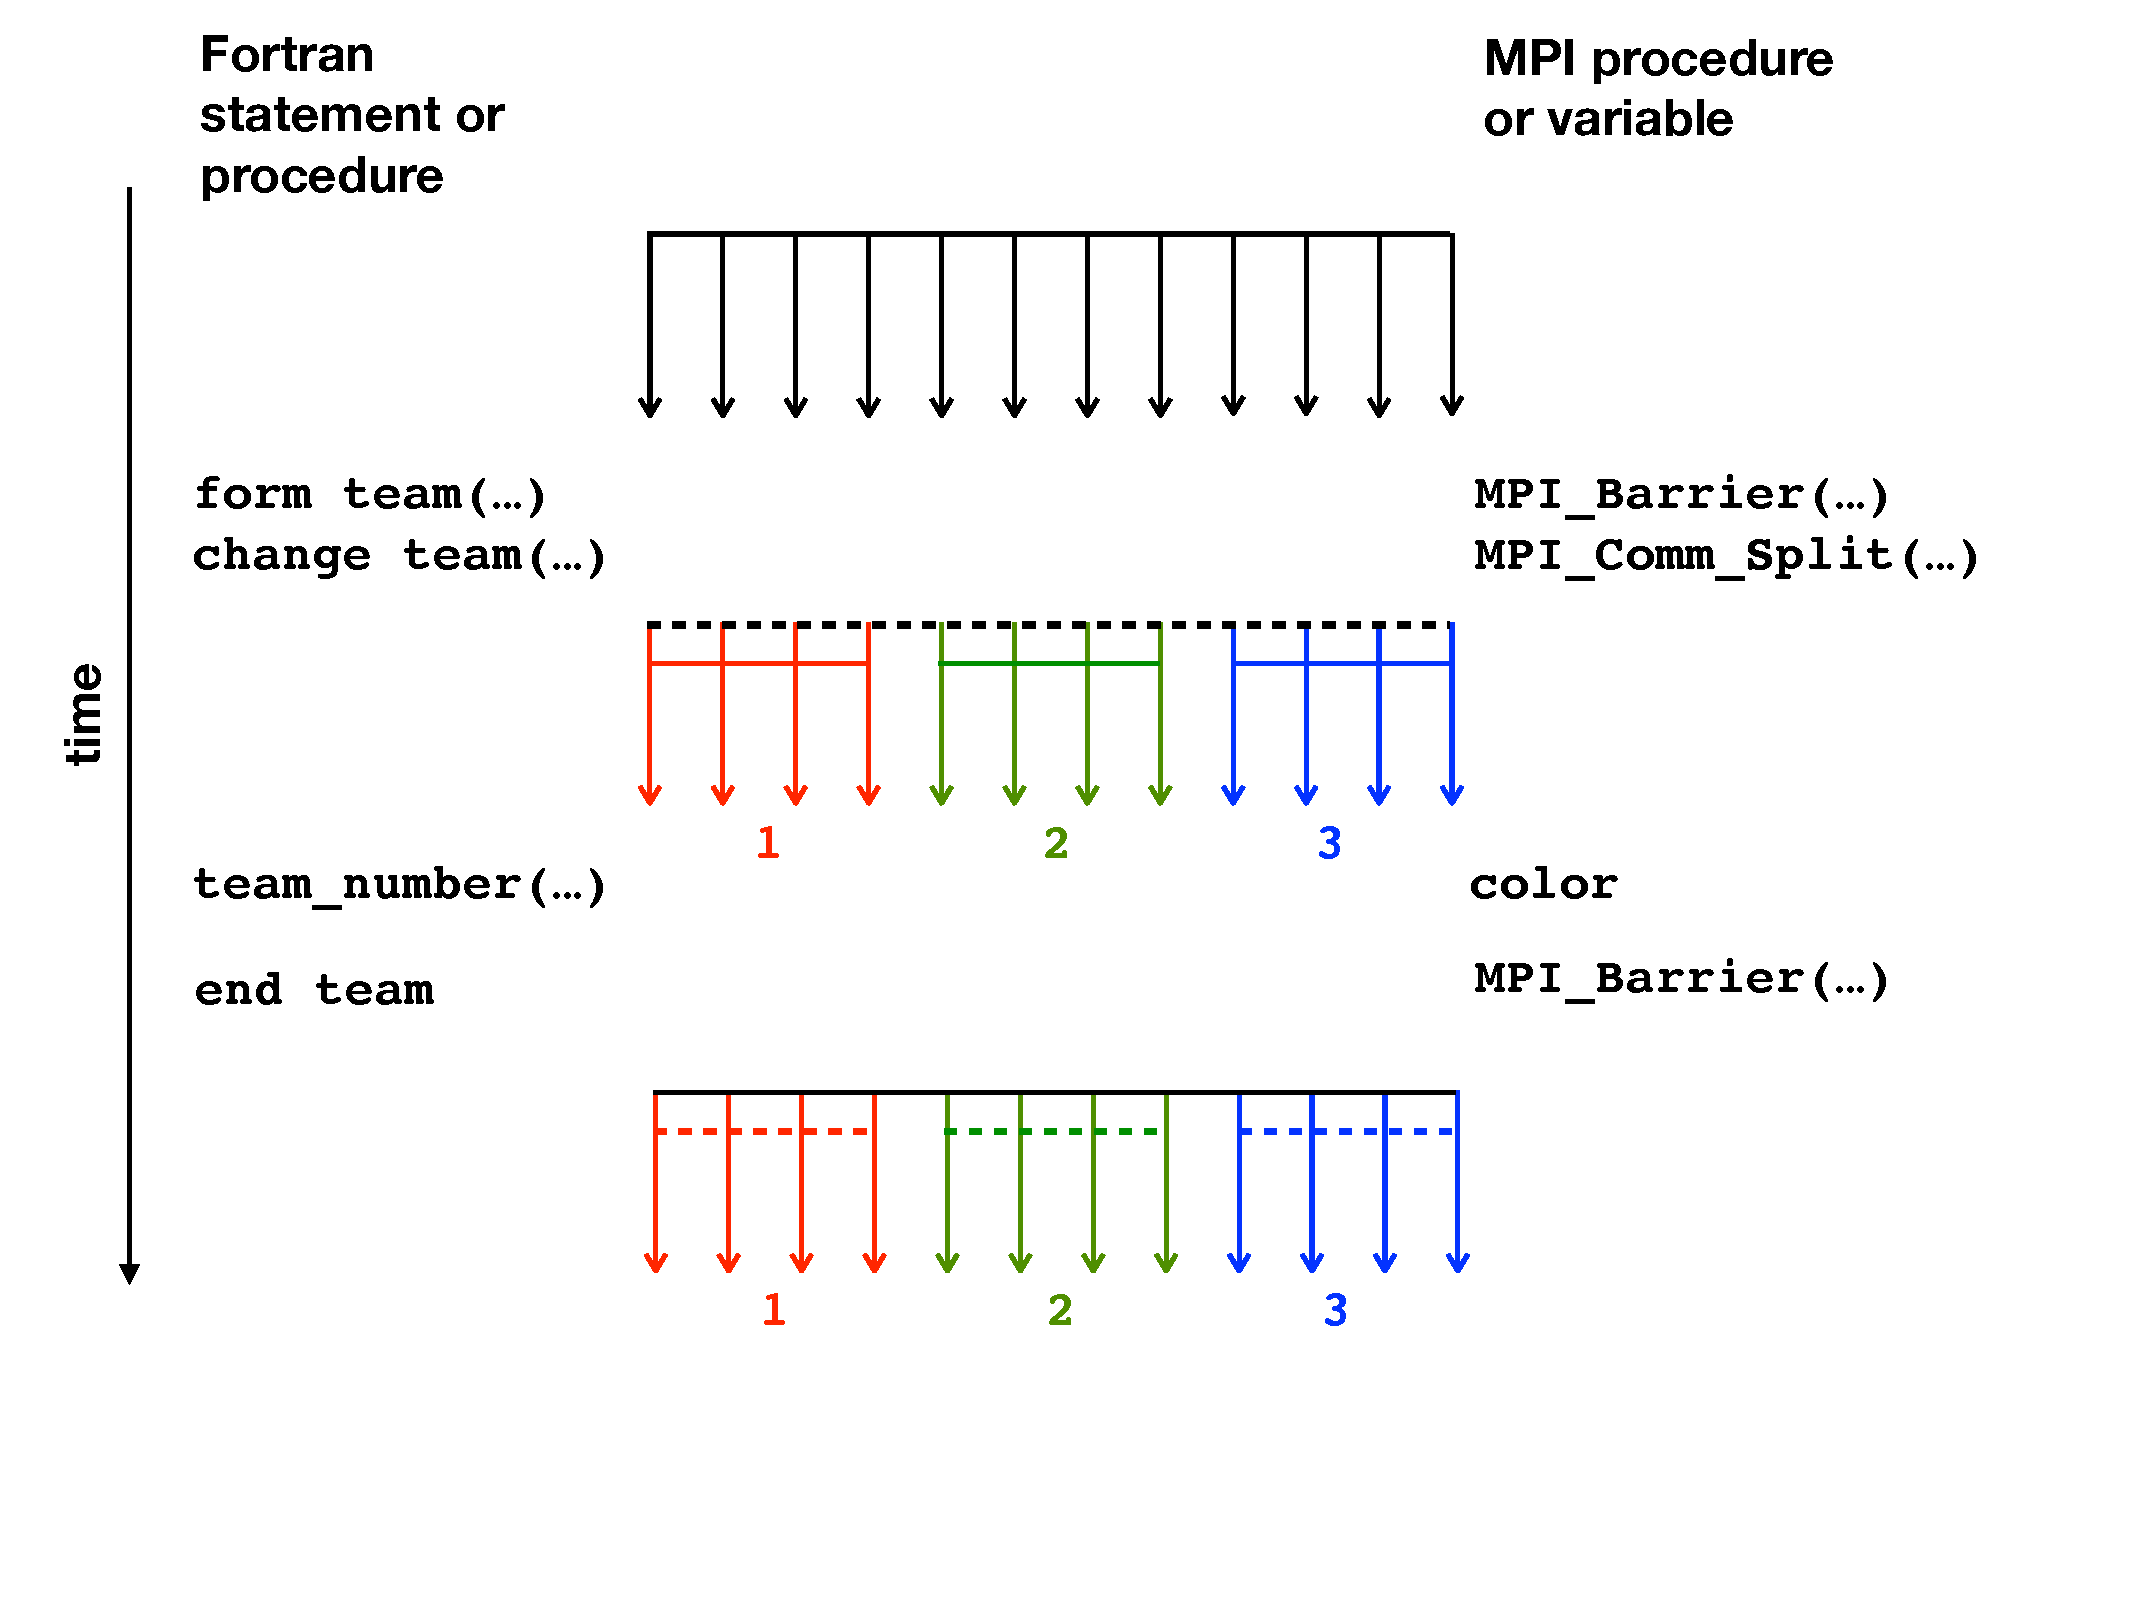
\includegraphics[width=0.7\textwidth]{figures/teams}
\vspace{-36pt}
\caption{Schematic depiction of a Fortran program executing over time
  (left axis) in 12 images (top) that communicate with each other through global means (black horizontal bar) and later communicating within subgroups (colored horizontal bars).  Horizontal lines represent the communication mechanisms (default=solid, optional=dashed).  Fortran concepts or on the left.  The underlying \gls{mpi} concepts are the right.\label{fig:teams}}
\end{figure*}
%

\begin{figure*}
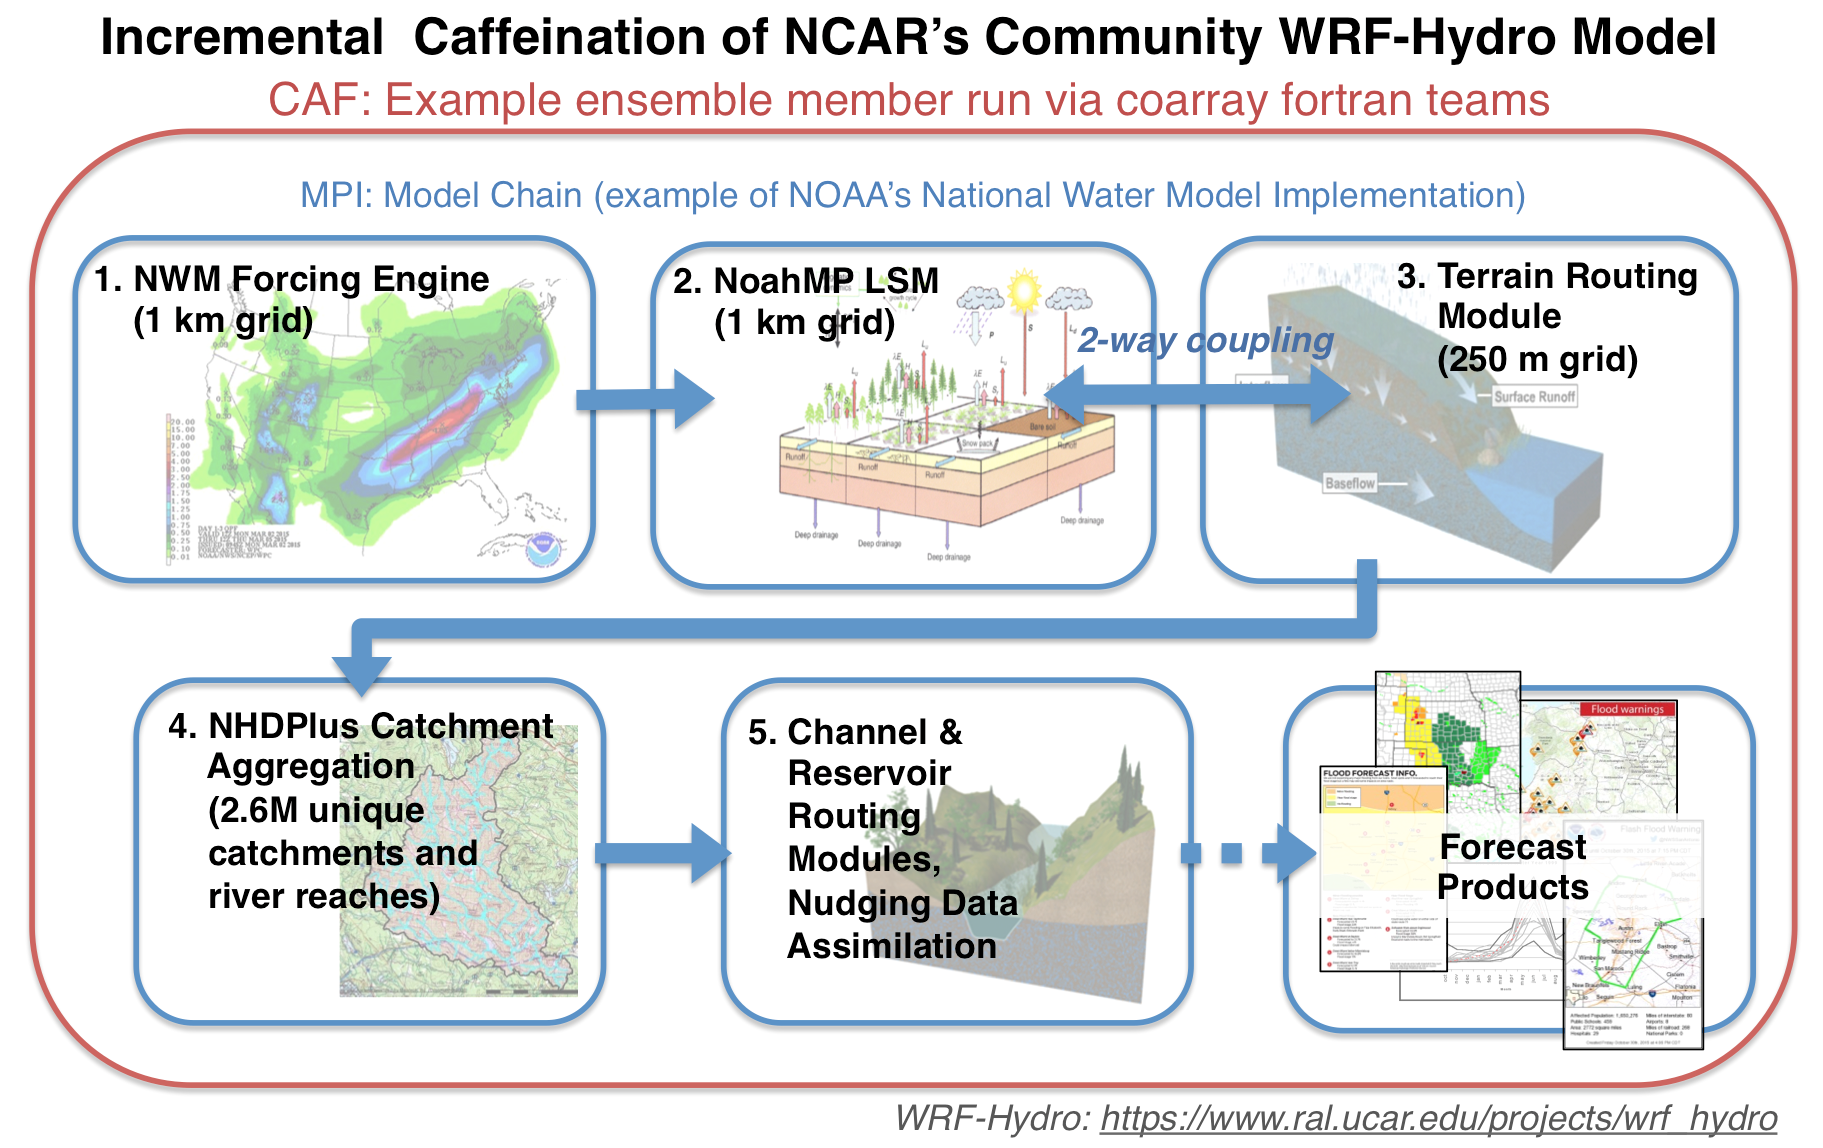
\includegraphics[width=0.7\textwidth]{figures/WRF-Hydro-caf-ens-model_chain.png}
\vspace{-7pt}
\caption{Caffeination of NCAR's WRF-Hydro model using coarray Fortran (CAF)
  teams. Specific example components of  NOAA's National Water
  Model are shown. Independent CAF teams run under a single Fortran executable are represented by the different colors
  (MPI terminology) in the stack.  Teams run separate instances
  (ensemble members) of the WRF-Hydro model chain to enable ensemble
  simulation and forecasting. The work presented  here supports for ``partial model caffeination'' with grouped
  parallelism (CAF teams): the underlying WRF-Hydro Model Chain
  originally under MPI can be transitioned incrementally towards CAF
  over time\label{fig:caffeinate-wrf-hydro}}
\end{figure*}
%

For illustrative purposes, we include two teams unit tests in
Figures~\ref{fig:get-team-test}--\ref{fig:team-number-test}.  These tests use a block distribution of images,
dividing the initial team into three new teams, each with the same number of images except that a number of
have one extra and the number of such images equals the remainder of integer division of the total
number imagesa by the number of teams.

\section{Discussion of Results}\label{sec:discussion}
\subsection{\gls{wrf-hydro}: Ensemble Simulation}
\gls{wrf-hydro} is a community hydrologic modeling system that provides a parallel-computing
framework for coupling Numerical Weather Prediction models (Figure \ref{fig:caffeinate-wrf-hydro}a), land surface models
(Figure \ref{fig:caffeinate-wrf-hydro}b), and a suite of hydrologic routing modules that handle spatial water redistribution
via surface (overland) flow (Figure \ref{fig:caffeinate-wrf-hydro}c), subsurface (soil column) flow (Figure \ref{fig:caffeinate-wrf-hydro}c),
baseflow (deep groundwater, \ref{fig:caffeinate-wrf-hydro}d), and stream channel transport
(Figure \ref{fig:caffeinate-wrf-hydro}e)~\cite{gochisEtal2014}.

While originally developed to couple land hydrology to the atmospheric processes of
the WRF model, WRF-Hydro is most commonly run in ``offline'' mode where it is one-way
coupled to (forced by) prescribed upper boundary (weather)
conditions (\ref{fig:caffeinate-wrf-hydro}). The chief example is NOAA's operational
National Water Model (NWM) ~\cite{noaa2016}; a special configuration of
WRF-Hydro which provides real-time analysis and forecasts of
hydrologic states over the contiguous U.S (\ref{fig:caffeinate-wrf-hydro}). Here we

Ensemble forecasting and ensemble data assimilation are active and
growing areas of research with WRF-Hydro. Running ensembles under a
single executable and job submission on HPC platforms as shown in
\ref{fig:caffeinate-wrf-hydro} can greatly reduce the amount
of labor involved in designing workflows and can open up new
possibilities for improving data flows and optimizing ensemble run
performance.

\begin{figure*}
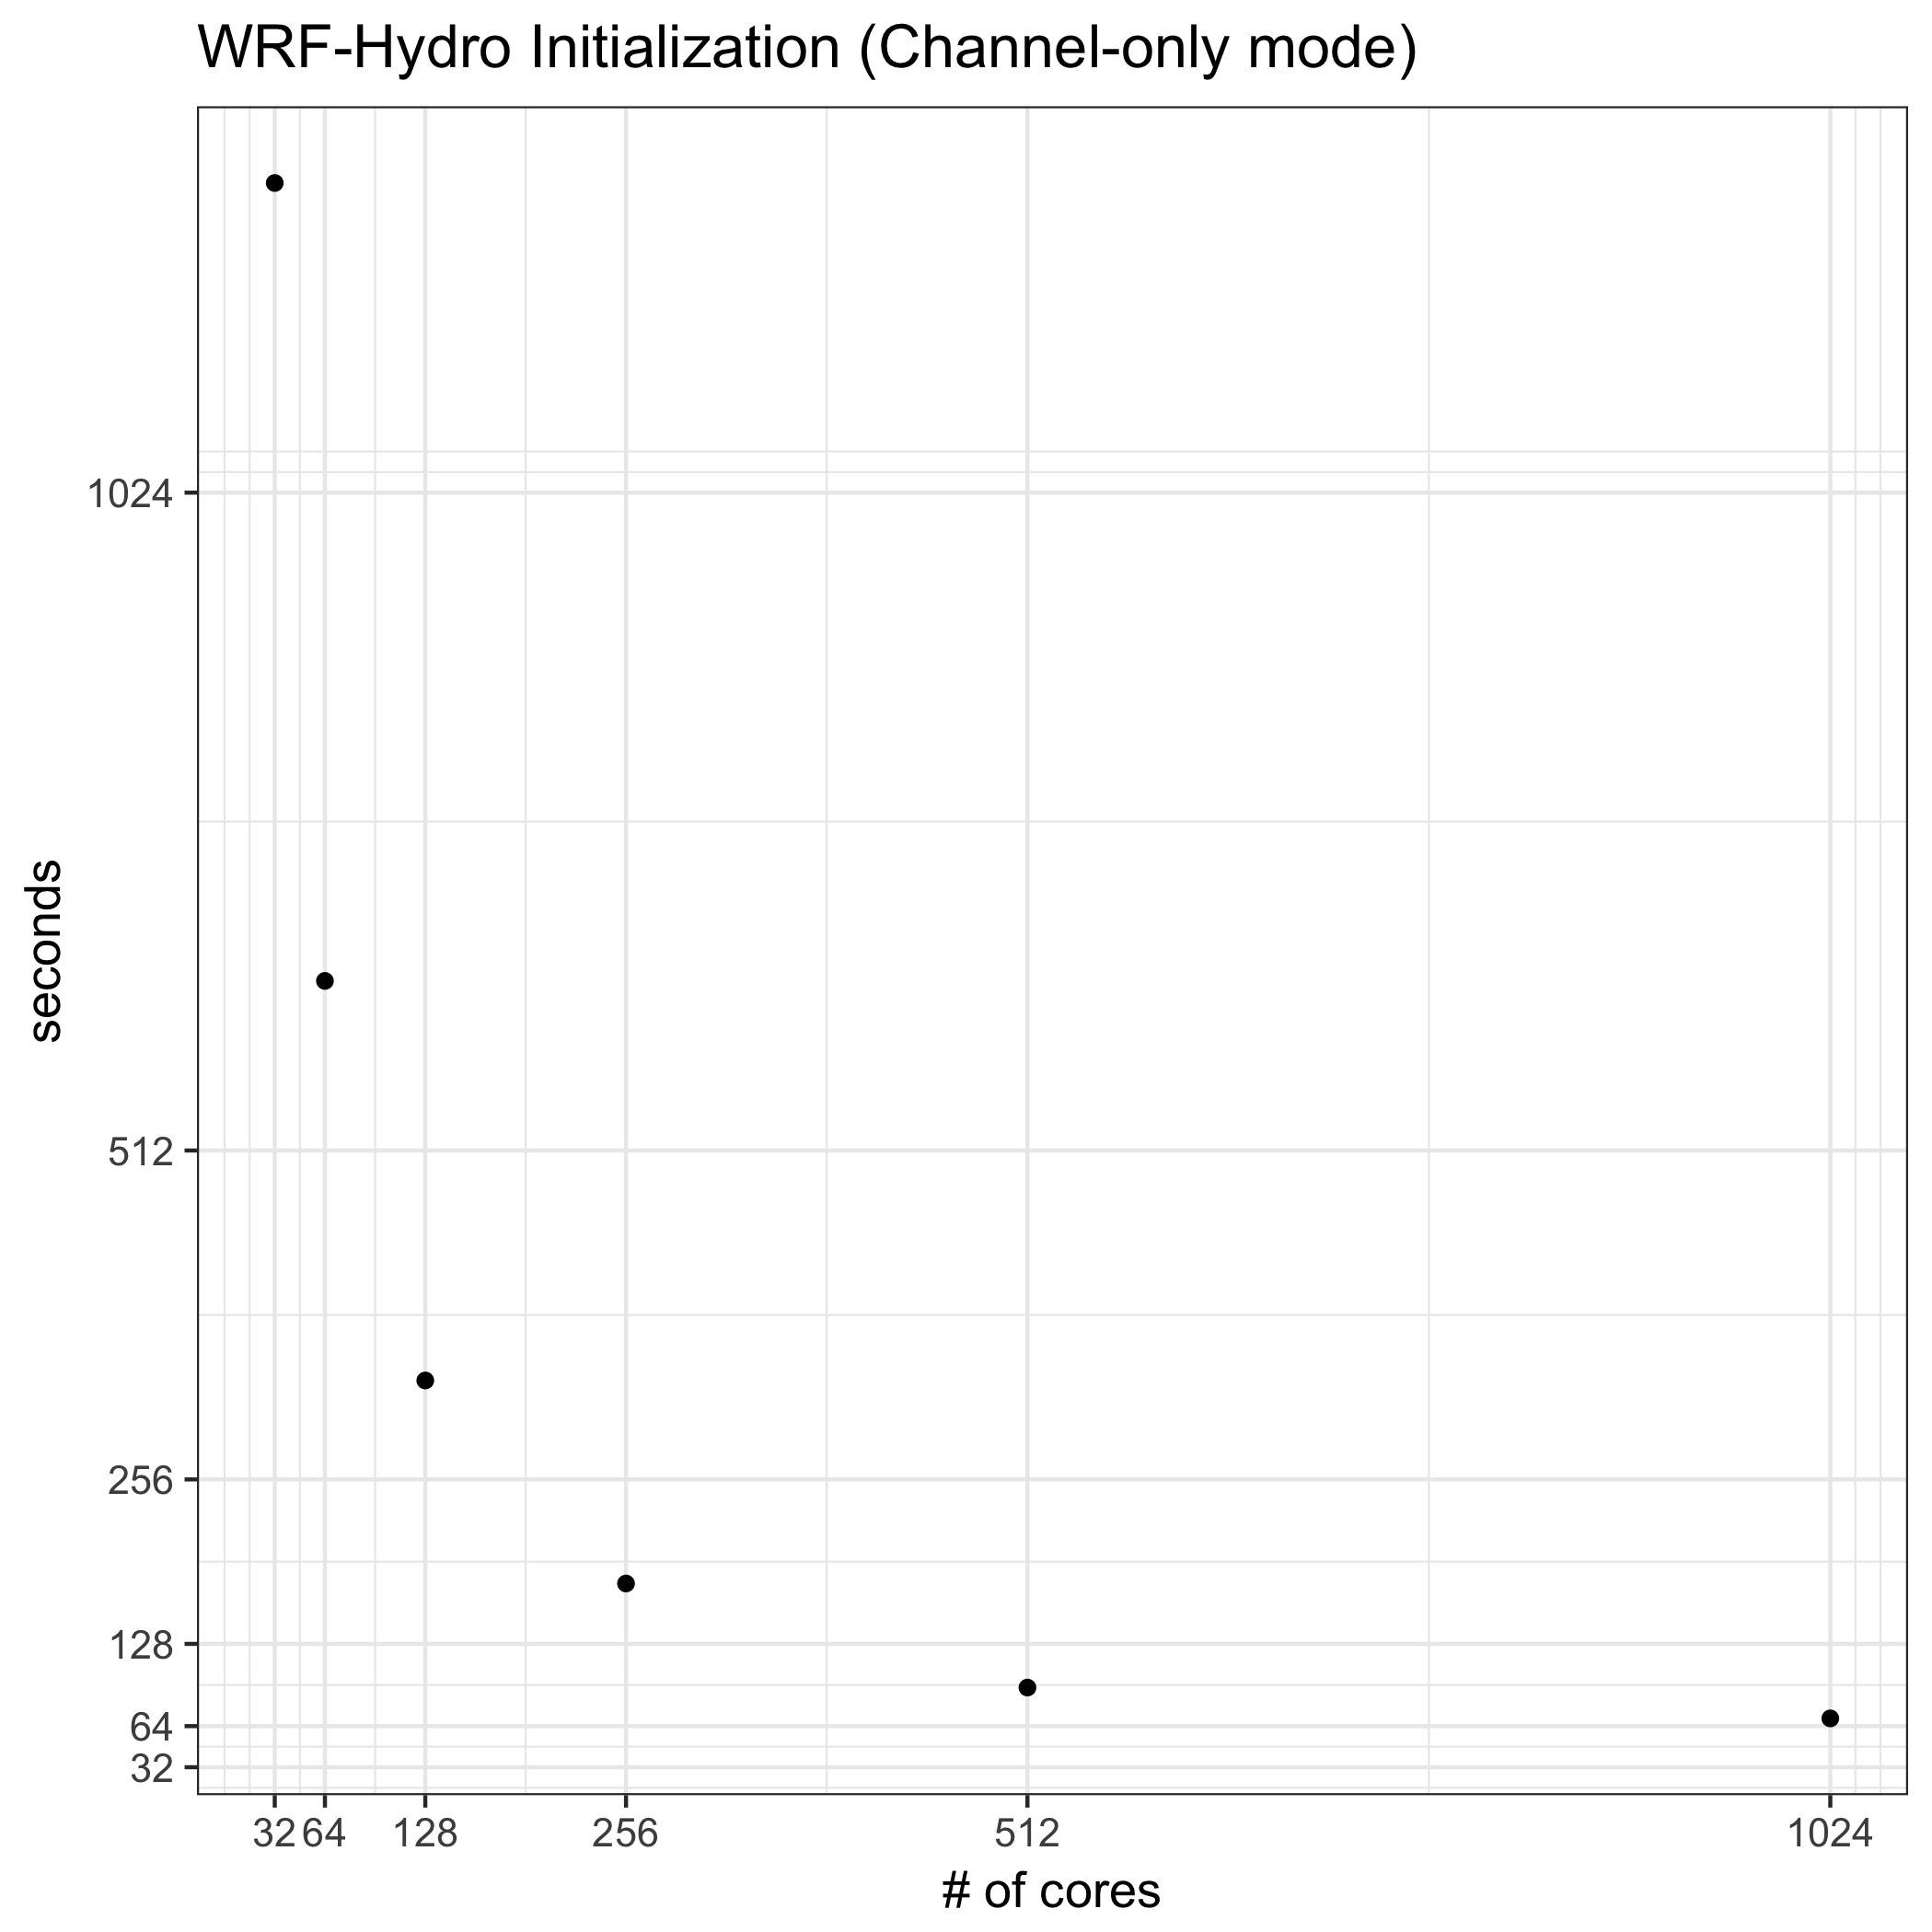
\includegraphics[width=0.7\textwidth]{figures/init_timing_linear.png}
\vspace{-7pt}
\caption{Scaling of the channel-only model initialization time to
  support calculation of Amdhal's law for estimating potential of
  saved compuation times \label{fig:wrf-hydro-init-scaling}}
\end{figure*}

Particularly, we plan to investigate restructuring the code to perform
model initialization which is shared over all ensemble members using
the full number of images prior to forming teams. Amortizing common
model initialization across all available computational resources
rather than repeating common aspects of the initialization in each
ensemble member using only that member's fraction of the resources has
the potentital to provide notable computational savings for
ensemble model runs where initialization comprises a large fraction of
the total run time. Such an example is in the production run of the
National Water Model short-term forecasts. Here we are currently
researching the possibility of moving from the current deterministic
(single ensemble member) model run to an ensemble run for the stream
channel submodel run in isolation. Scaling of the
initialization of the channel-only model is presented in
\ref{fig:wrf-hydro-init-scaling}. If 50 ensemble members are run concurrently with
teams occupying 20 cores each, the initialization speedup will be
approximately 20x. Currently, for the short-range forecasts,
initialization requires approximately 50\% of the run time on
NCAR's yellowstone computer and greater than that on NOAA's WCOSS
system~\cite{yuetal2017}. These numbers are
similar for the channel-only model. In our proposed application for an ensemble size of 50, we estimate that
approximately half the runtime ($f=.5$) can be sped up by a factor of
about 20 ( $S_f=20$), based on \ref{fig:wrf-hydro-init_scaling}. From
these estimates, Amdhal\'s law yields a total speedup
of 1.9:

\begin{equation}
S = 1 / { f/S_f + (1-f) } = 1 / (.5/20 + (1-.5)) = 1.9
\end{equation}

Obtaining speed up of 1.9 when running ensembles by using CAF
teams and restructuring the initialization would be welcome news in the
operational (NWM) setting where it would help either reduce forecast latency
or allow reduction of 24\/7 dedicated resources.

In the application of teams to WRF Hydro, the main WRF-Hydro program is wrapped in a loop
over the individual ensemble members. The number of images per team and the
 number of ensemble members are specified in a namelist. Along with
 the number of available images, these parameters determine how many
 teams are formed and which teams handle which ensemble members. It is
 worth noting several details of separate runs which may potentially need altering
 when running ensembles via teams: 1) \texttt{MPI\_INIT}, 2) \texttt{MPI\_FINALIZE}, 3)
 variable initialization and allocation, 4) \texttt{STOP}.

\subsection{A language extension}
Discuss \lstinline|get_communicator|

\section{Conclusions and Future Work}\label{sec:conclusions}

%%%
%%% Sample tables
%%%

%\begin{table}
%  \caption{Frequency of Special Characters}
%  \label{tab:freq}
%  \begin{tabular}{ccl}
%    \toprule
%    Non-English or Math&Frequency&Comments\\
%    \midrule
%    \O & 1 in 1,000& For Swedish names\\
%    $\pi$ & 1 in 5& Common in math\\
%    \$ & 4 in 5 & Used in business\\
%    $\Psi^2_1$ & 1 in 40,000& Unexplained usage\\
%  \bottomrule
%\end{tabular}
%\end{table}

%\begin{table*}
%  \caption{Some Typical Commands}
%  \label{tab:commands}
%  \begin{tabular}{ccl}
%    \toprule
%    Command &A Number & Comments\\
%    \midrule
%    \texttt{{\char'134}author} & 100& Author \\
%    \texttt{{\char'134}table}& 300 & For tables\\
%    \texttt{{\char'134}table*}& 400& For wider tables\\
%    \bottomrule
%  \end{tabular}
%\end{table*}
% end the environment with {table*}, NOTE not {table}!

%It is strongly recommended to use the package booktabs~\cite{Fear05}
%and follow its main principles of typography with respect to tables:
%\begin{enumerate}
%\item Never, ever use vertical rules.
%\item Never use double rules.
%\end{enumerate}
%It is also a good idea not to overuse horizontal rules.


%%%
%%% Sample figures
%%%

%\begin{figure}
%\includegraphics{fly}
%\caption{A sample black and white graphic.}
%\end{figure}

%\begin{figure}
%\includegraphics[height=1in, width=1in]{fly}
%\caption{A sample black and white graphic
%that has been resized with the \texttt{includegraphics} command.}
%\end{figure}

%\begin{figure*}
%\includegraphics{flies}
%\caption{A sample black and white graphic
%that needs to span two columns of text.}
%\end{figure*}
%
%\begin{figure}
%\includegraphics[height=1in, width=1in]{rosette}
%\caption{A sample black and white graphic that has
%been resized with the \texttt{includegraphics} command.}
%\end{figure}

%\end{document}  % This is where a 'short' article might terminate



%\appendix
%Appendix A
%\section{Teams unit tests}
% This next section command marks the start of
% Appendix B, and does not continue the present hierarchy

\begin{figure*}
  \lstinputlisting{figures/tests/get-team.f90}
  \caption{A unit test for the get-team function.\label{fig:get-team-test}}
\end{figure*}

%\begin{figure*}
%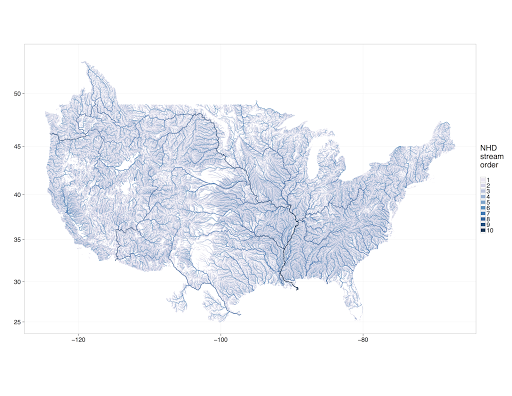
\includegraphics[width=0.7\textwidth]{figures/hydro-map}
%\vspace{-36pt}
%\caption{Sample \gls{wrf-hydro} simulation domain.}
%\end{figure*}
%

\begin{figure*}
  \lstinputlisting{figures/tests/team-number.f90}
  \caption{A unit test for the team-number function.\label{fig:team-number-test}}
\end{figure*}

\begin{acks}
The first author would like to thank the Visitor Programs of the Computational Information Systems Laboratory and the Research Applications Laboratory of \gls{ncar} for travel support for a visit during which much of the work presented in this paper was performed.

%  The work is
%  supported by the \grantsponsor{GSxxxxx}{National
%  Science Foundation China}{http://dx.doi.org/zz.yyyyy/xxxxx} under Grant
%  No.:~\grantnum{GSxxxxx}{yyyyyyy}

\end{acks}
